% !TeX spellcheck = en_GB
\documentclass[AERbeamer%              style
              ,optEnglish%            language
              %,handout%               deactivate animation
              ,optBiber%               bibliography tool
              ,optBibstyleAlphabetic%
              ,optBeamerClassicFormat% 4:3 format
              %,optBeamerWideFormat%   16:9 format
              ]{AERlatex}%
\setbeameroption{show notes}% Show all notes
%
% Set paths
\graphicspath{{figures_lecture_2/}}%
\addbibresource{literature.bib}%
%
% Package Imports
%\usepackage{media9}
\usepackage{graphicx}
\usepackage{multimedia}
\usepackage{subcaption}
\usepackage{amsmath}
%
% set meta data
\title{Probabilistic Programming for Scientific Discovery}%
\subtitle{Lecture 2}
\author{Ludger Paehler}% (optional)
\date{\AERutilsDate{29}{7}{2020}}% (optional)
\institute{Lviv Data Science Summer School}% (optional)
%
% Setup of header and footer
\AERbeamerSetupHeader{\AERlayoutHeaderCDChair}%
\AERbeamerSetupFooterCD%
%\AERbeamerSetupFooterSlideNumberOnly%
%
\begin{document}%
%
% Start with titlepage
\AERbeamerTitlePageDefault%
%
%\begin{frame}{Title of Slide}{Subtitle of Slide}%
%    \blindtext%
%\end{frame}%
%

% Slide 0: Table of Contents
\begin{frame}{Table of Contents}{}%
    % Contents
    \tableofcontents
\end{frame}%


% Approaches to Inference, the Core of every respectable Probabilistic Programming Framework
\section{Approaches to Inference - the Inference Engines}


% Introductory slide to show how everything centers around the inference algorithm library in probabilistic programming
\begin{frame}[c]{Approaches to Inference - the Inference Engines}
    % Two columns, explanation on the left probabilistic programming system explanation on the right
    \begin{columns}[T]
        % Explaining the typical construction of a PPS
        \begin{column}{0.48\textwidth}
            \centering
            \begin{itemize}
                \item A typical probabilistic programming system consists of:
                \begin{itemize}
                    \item A domain-specific language (DSL), which enables the user to express his model using the language-specific primitives
                    \item Provides a library of inference algorithms, which enable inference on probabilistic models definable in the
                          DSL.
                    \item Prevalent Monte-Carlo and variational inference approaches have their own specific sets of strength, it is
                          hence important to understand the inference algorithms one utilizes
                \end{itemize}
            \end{itemize}
        \end{column}
        % Illustration of a typical PPS
        \begin{column}{0.48\textwidth}
            \centering
            \begin{figure}
                \centering
                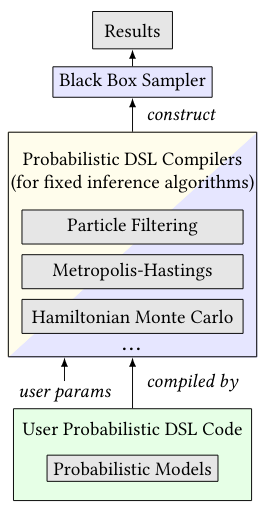
\includegraphics[width=0.4\textwidth]{TypicalPPS.png}
                \caption{Structure of a typical probabilistic programming system. Source: \textit{Gen: A General-Purpose Probabilistic Programming Systems with Programmable Inference}}
            \end{figure}
        \end{column}
    \end{columns}
\end{frame}


% Subsection for Monte-Carlo algorithms of all flavours
\subsection{Monte-Carlo}


\subsubsection*{Hamiltonian Monte Carlo}
% Hamiltonian Monte-Carlo Slide 1
\begin{frame}[c]{Monte-Carlo Approaches to Inference}{Hamiltonian Monte-Carlo \footnote{Neal, R.M., 2011. MCMC using Hamiltonian dynamics. Handbook of markov chain monte carlo, 2(11), p.2.}}
    \centering
    \begin{itemize}
        \item Hamiltonian Monte-Carlo 1
    \end{itemize}
\end{frame}


% Hamiltonian Monte-Carlo Slide 2
\begin{frame}[c]{Monte-Carlo Approaches to Inference}{Hamiltonian Monte-Carlo}
    \centering
    \begin{itemize}
        \item Hamiltonian Monte-Carlo 2
    \end{itemize}
\end{frame}


% Hamiltonian Monte-Carlo Slide 3
\begin{frame}[c]{Monte-Carlo Approaches to Inference}{Hamiltonian Monte-Carlo}
    \centering
    \begin{itemize}
        \item Hamiltonian Monte-Carlo 3
    \end{itemize}
\end{frame}


% Hamiltonian Monte-Carlo Slide 4
\begin{frame}[c]{Monte-Carlo Approaches to Inference}{Hamiltonian Monte-Carlo}
    \centering
    \begin{itemize}
        \item Hamiltonian Monte-Carlo 4
    \end{itemize}
\end{frame}



\subsubsection*{Random-Walk Metropolis Hastings}
% Random-Walk Metropolis Hastings Slide 1
\begin{frame}[c]{Monte-Carlo Approaches to Inference}{Random-Walk Metropolis Hastings \footnote{Gelman, A., Carlin, J.B., Stern, H.S., Dunson, D.B., Vehtari, A. and Rubin,
                                                                                                D.B., 2013. Bayesian data analysis. CRC press.}
                                                                                      \footnote{Gilks, W.R. and Richardson, S., S. and Spiegelhalter, D.(1996). Markov chain
                                                                                                Monte Carlo in practice. London, UK: Chapman k Hall/CRC.}}
    \centering
    \begin{itemize}
        \item Random-Walk Metropolis Hastings 1
    \end{itemize}
\end{frame}


% Random-Walk Metropolis Hastings Slide 2
\begin{frame}[c]{Monte-Carlo Approaches to Inference}{Random-Walk Metropolis Hastings}
    \centering
    \begin{itemize}
        \item Random-Walk Metropolis Hastings 2
    \end{itemize}
\end{frame}


% Random-Walk Metropolis Hastings Slide 3
\begin{frame}[c]{Monte-Carlo Approaches to Inference}{Random-Walk Metropolis Hastings}
    \centering
    \begin{itemize}
        \item Random-Walk Metropolis Hastings 3
    \end{itemize}
\end{frame}


% Random-Walk Metropolis Hastings Slide 4
\begin{frame}[c]{Monte-Carlo Approaches to Inference}{Random-Walk Metropolis Hastings}
    \centering
    \begin{itemize}
        \item Random-Walk Metropolis Hastings 4
    \end{itemize}
\end{frame}



\subsubsection*{Stochastic-Gradient Langevin Dynamics}
% Stochastic-Gradient Langevin Dynamic Monte-Carlo Slide 1
\begin{frame}[c]{Monte-Carlo Approaches to Inference}{Stochastic-Gradient Langevin Dynamics \footnote{Welling, M. and Teh, Y.W., 2011. Bayesian learning via stochastic gradient Langevin
                                                                                                      dynamics. In Proceedings of the 28th international conference on machine learning
                                                                                                      (ICML-11) (pp. 681-688).}
                                                                                            \footnote{Brosse, N., Durmus, A. and Moulines, E., 2018. The promises and pitfalls of stochastic
                                                                                                      gradient Langevin dynamics. In Advances in Neural Information Processing Systems (pp. 8268-8278).}}
    \centering
    \begin{itemize}
        \item Stochastic-Gradient Langevin Dynamics 1
    \end{itemize}
\end{frame}


% Stochastic-Gradient Langevin Dynamic Monte-Carlo Slide 2
\begin{frame}[c]{Monte-Carlo Approaches to Inference}{Stochastic-Gradient Langevin Dynamics}
    \centering
    \begin{itemize}
        \item Stochastic-Gradient Langevin Dynamics 2
    \end{itemize}
\end{frame}


% Stochastic-Gradient Langevin Dynamic Monte-Carlo Slide 3
\begin{frame}[c]{Monte-Carlo Approaches to Inference}{Stochastic-Gradient Langevin Dynamics}
    \centering
    \begin{itemize}
        \item Stochastic-Gradient Langevin Dynamics 3
    \end{itemize}
\end{frame}


% Stochastic-Gradient Langevin Dynamic Monte-Carlo Slide 4
\begin{frame}[c]{Monte-Carlo Approaches to Inference}{Stochastic-Gradient Langevin Dynamics}
    \centering
    \begin{itemize}
        \item Stochastic-Gradient Langevin Dynamics 4
    \end{itemize}
\end{frame}



% Variational Inference
\subsection{Variational Inference}

\subsubsection*{Classical Variational Inference}
% Variational Inference Slide 1
\begin{frame}[c]{Variational Approaches to Inference}{Variational Inference \footnote{Blei, D.M., Kucukelbir, A. and McAuliffe, J.D., 2017. Variational inference: A
                                                                                      review for statisticians. Journal of the American statistical Association, 112(518),
                                                                                      pp.859-877.}
                                                                            \footnote{Zhang, C., Bütepage, J., Kjellström, H. and Mandt, S., 2018. Advances in variational inference.
                                                                                      IEEE transactions on pattern analysis and machine intelligence, 41(8), pp.2008-2026.}
                                                                            \footnote{Salimans, T., Kingma, D. and Welling, M., 2015, June. Markov chain monte carlo and variational
                                                                                      inference: Bridging the gap. In International Conference on Machine Learning (pp. 1218-1226).}}
    \centering
    \begin{itemize}
        \item Rephrases the problem from a Monte-Carlo sampling, which requires significant computation but converges to the true posterior to one,
              where we propose a family of distributions to then be optimized to be as close to the true posterior as possible using the Kullback-Leibler
              divergence
        \begin{itemize}
            \item An approach to approximate densities, whereas MCMC is a tool to simulate from densities
            \item Underestimates the variance of the posterior density
        \end{itemize}
        \item Suited for large problems and problems of high complexity, where a Monte-Carlo inference would be computationally intractable
        \item Possible to make variational inference more efficient with a few markov chain monte carlo samples beforehand for a better initialization
    \end{itemize}
\end{frame}


% Variational Inference Slide 2
\begin{frame}[c]{Variational Approaches to Inference}{Variational Inference}
    \centering
    \begin{itemize}
        \item Positing the family of approximate densities $\mathcal{D}$ and optimizing for the Kullback-Leibler divergence
        \begin{equation*}
            q^{\star}(z) = \underset{q(z) \in \mathcal{D}}{\arg \min} \text{KL}(q(z) || p(z|x))
        \end{equation*}
        \item The reach of the density family $\mathcal{D}$ governs the complexity of the optimization problem.
        \item The Kullback-Leibler divergence can be decomposed into
        \begin{equation*}
            \text{KL}(q(z) || p(z|x)) = \mathbb{E}[\log q(z)] - \mathbb{E}[\log p(z|x)]
        \end{equation*}
        \item The Kullback-Leibler divergence is intractable for complex distributions, we hence define a surrogate objective
              called the evidence lower-bound (ELBO). The ELBO is the negative KL divergence plus a constant
        \begin{equation*}
            \text{ELBO}(q) = \mathbb{E}[\log p(z, x)] - \mathbb{E}[\log q(z)]
        \end{equation*}
    \end{itemize}
\end{frame}


% Variational Inference Slide 3
\begin{frame}[c]{Variational Approaches to Inference}{Variational Inference}
    \centering
    \begin{itemize}
        \item We hence have
        \begin{equation*}
            \max \text{ ELBO} \sim \min \text{ KL}
        \end{equation*}
        \item The exact relation between the KL divergence measure and the surrogate objective is then
        \begin{equation*}
            \log p(x) = \text{KL}(q(z) || p(z|x)) + \text{ELBO}(q)
        \end{equation*}
        \item The most commonly used families of distributions belong to the mean-field variational family of distributions
        \begin{itemize}
            \item Beware, the mean-field family cannot capture correlations between marginal densities!
        \end{itemize}
        \begin{equation*}
            q(z) = \prod^{m}_{j=1} q_{j}(z_{j})
        \end{equation*}
        \item There exists work though, which approximates more complex distributions \footnote{Saul, L.K. and Jordan, M.I., 1996. Exploiting tractable substructures in intractable
                                                                                                networks. In Advances in neural information processing systems (pp. 486-492).}
                                                                                      \footnote{Barber, D. and Wiegerinck, W., 1999. Tractable variational structures for approximating
                                                                                                graphical models. In Advances in Neural Information Processing Systems (pp. 183-189).}
    \end{itemize}
\end{frame}


% Variational Inference Slide 4
\begin{frame}[c]{Variational Approaches to Inference}{Variational Inference}
    \centering
    \begin{figure}
        \centering
        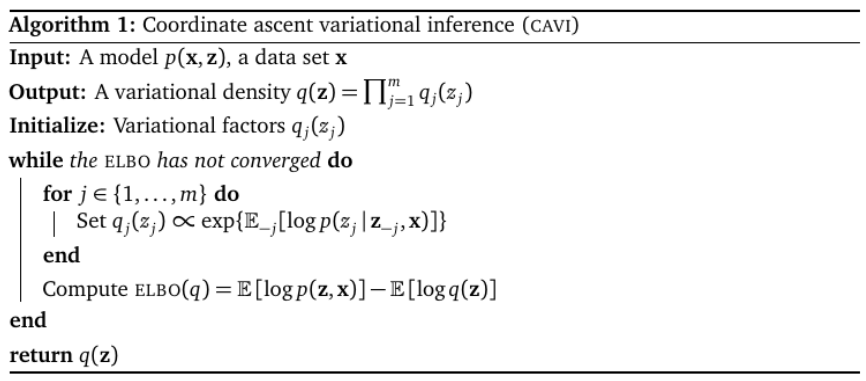
\includegraphics[width=0.7\textwidth]{VICAVIAlgo.png}
    \end{figure}
    \begin{itemize}
        \item But CAVI needs to iterate through the entire dataset for one iteration, hence motivating the use of stochastic approximations
    \end{itemize}
\end{frame}


% Variational Inference Slide 5
\begin{frame}[c]{Variational Approaches to Inference}{Variational Inference}
    \centering
    \begin{figure}
        \centering
        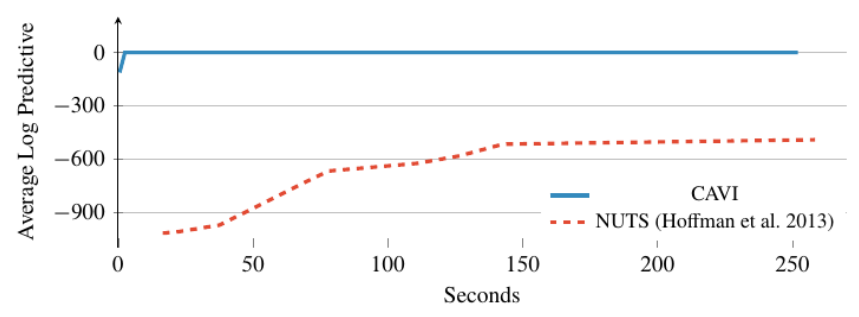
\includegraphics[width=0.5\textwidth]{VICAVIvsHMC.png}
        \caption{CAVI vs HMC using a NUTS sampler.}
    \end{figure}
    \begin{figure}
        \centering
        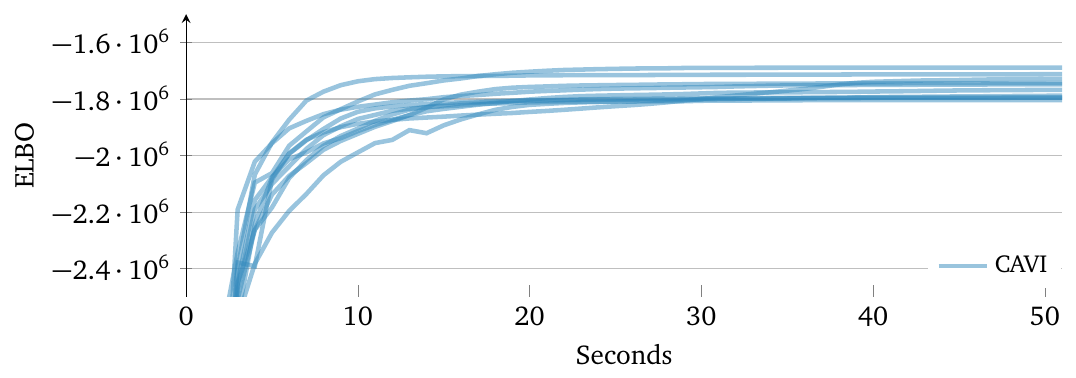
\includegraphics[width=0.5\textwidth]{VICAVIELBO.png}
        \caption{CAVI with different initializations.}
    \end{figure}
\end{frame}



\subsubsection*{Stochastic Variational Inference}
% Stochastic Variational Inference Slide 1
\begin{frame}[c]{Variational Approaches to Inference}{Stochastic Variational Inference \footnote{Hoffman, M.D., Blei, D.M., Wang, C. and Paisley, J., 2013. Stochastic variational
                                                                                                 inference. The Journal of Machine Learning Research, 14(1), pp.1303-1347.}
                                                                                       \footnote{Robbins, H. and Monro, S., 1951. A stochastic approximation method. The annals of 
                                                                                                 mathematical statistics, pp.400-407.}}
    \centering
    \begin{itemize}
        \item Stochastic variational inference (SVI) combines the natural gradients of Amari with the stochastic optimization of
              Robbins and Monroe
        \item The algorithm form of SVI can be sketched in the following way
        \begin{enumerate}
            \item Subsample one or more data points from the data
            \item Analyze the subsample using the current variational parameters
            \item Implement a closed-form update of the variational parameters
            \item Repeat
        \end{enumerate}
        \item The used natural gradients alter the parameter space s.t. the same distance in different directions
              alters the symmetrized KL divergence by equal amounts
        \item Natural gradients are easier to compute than Euclidian gradients
        \item Suitable for extreme-scale applications, who don't need to fit in memory
    \end{itemize}
\end{frame}


% Stochastic Variational Inference Slide 2
\begin{frame}[c]{Variational Approaches to Inference}{Stochastic Variational Inference}
    \centering
    \begin{itemize}
        \item Stochastic optimization then follows the cheaper natural gradients to find the maximum of the ELBO
        \item The sequence of step size for the optimization needs to obey the following condition meanwhile:
        \begin{equation*}
            \sum_{t} \epsilon_{t} = \infty; \quad \sum_{t} \epsilon^{2}_{t} < \infty
        \end{equation*}
        \item Writing the gradient of the ELBO as an expectation one can then computer Monte-Carlo estimates of the
              gradient and hence compute a few gradients before starting the actual SVI algorithm
        \item Has to make a few constraining assumptions for closed-form optimization:
        \begin{itemize}
            \item Each conditional is in an exponential family
            \item The variational distribution has to be in the same exponential family
        \end{itemize}
        \item Does not need to iterate over the complete dataset and only requires computation over local context for each iteration
    \end{itemize}
\end{frame}


% Stochastic Variational Inference Slide 3
\begin{frame}[c]{Variational Approaches to Inference}{Stochastic Variational Inference}
    \centering
    \begin{figure}
        \centering
        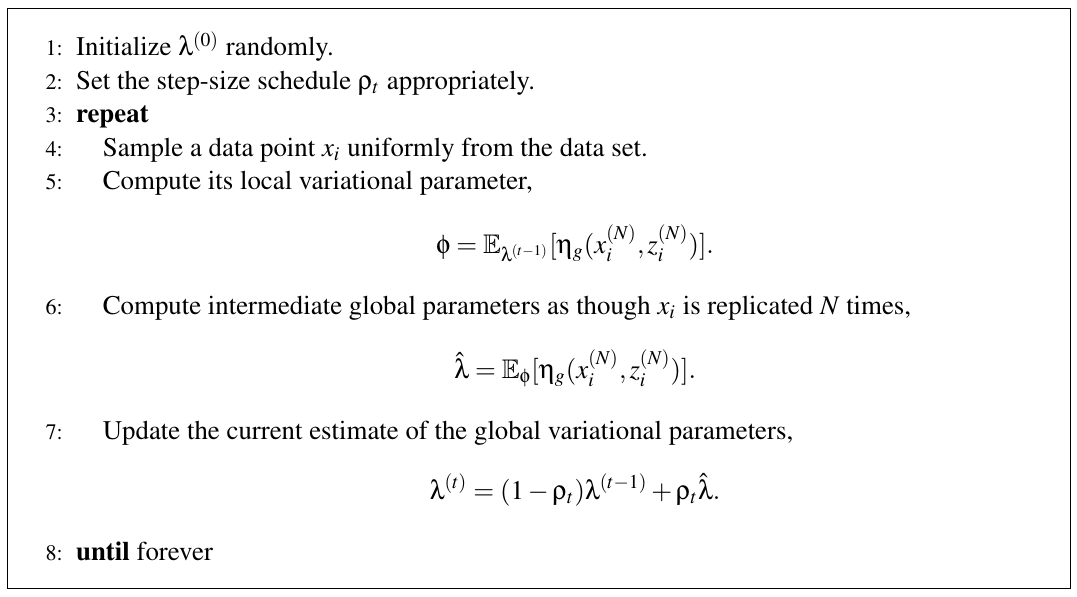
\includegraphics[width=0.8\textwidth]{VISVIAlgo.png}
    \end{figure}
\end{frame}


% Stochastic Variational Inference Slide 4
\begin{frame}[c]{Variational Approaches to Inference}{Stochastic Variational Inference}
    \centering
    \begin{columns}[T]
        \begin{column}{0.4\textwidth}
                More involved algorithm for a hierarchical dirichlet process topic model
                \begin{itemize}
                    \item Draw an infinite number of topics, $\beta_{k} \sim \text{Dirichlet}(\eta)$ for $k \in {1, 2, 3, \ldots}$
                    \item Draw corpus breaking proportions, $\nu_{k} \sim \text{Beta}(1, \omega)$ for $k \in {1, 2, 3, \ldots}$
                    \item For each document d:
                    \begin{itemize}
                        \item Draw document-level top indices
                        \item Draw document breaking proportions
                        \item For each word n:
                        \begin{itemize}
                            \item $\quad$ Draw topic assignment
                            \item $\quad$ Draw word
                        \end{itemize}
                    \end{itemize}
                \end{itemize}
        \end{column}
        \begin{column}{0.58\textwidth}
            \begin{figure}
                \centering
                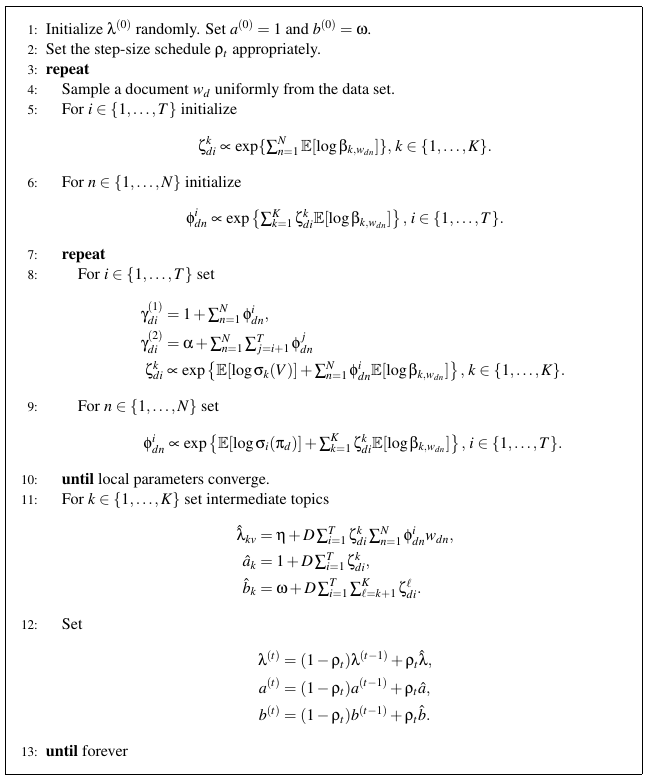
\includegraphics[width=0.7\textwidth]{VISVIforHDP.png}
            \end{figure}
        \end{column}
    \end{columns}
\end{frame}


% Stochastic Variational Inference Slide 5
\begin{frame}[c]{Variational Approaches to Inference}{Stochastic Variational Inference}
    Recap:
    \begin{itemize}
        \item Core idea: Use stochastic optimization to optimize the variational objective, following the noisy
              estimates of the natural gradient
        \item Adaptive learning rates can further accelerate the stochastic inference routine
        \item Can be used to further scale up recent advances
        \item Can benefit from further advances in stochastic optimization
    \end{itemize}
\end{frame}



\subsubsection*{Black-Box Variational Inference}
% Black-Box Variational Inference Slide 1
\begin{frame}[c]{Variational Approaches to Inference}{Black Box Variational Inference \footnote{Ranganath, R., Gerrish, S. and Blei, D., 2014, April. Black box
                                                                                                variational inference. In Artificial Intelligence and Statistics (pp. 814-822).}
                                                                                      \footnote{Chu, C., Minami, K. and Fukumizu, K., 2020. The equivalence between Stein
                                                                                                variational gradient descent and black-box variational inference. arXiv preprint arXiv:2004.01822.}}
    \centering
    \begin{itemize}
        \item Black Box Variational Inference 1
    \end{itemize}
\end{frame}


% Black-Box Variational Inference Slide 2
\begin{frame}[c]{Variational Approaches to Inference}{Black Box Variational Inference}
    \centering
    \begin{itemize}
        \item Black Box Variational Inference 2
    \end{itemize}
\end{frame}


% Black-Box Variational Inference Slide 3
\begin{frame}[c]{Variational Approaches to Inference}{Black Box Variational Inference}
    \centering
    \begin{columns}[T]
        \begin{column}{0.48\textwidth}
            \begin{figure}
                \centering
                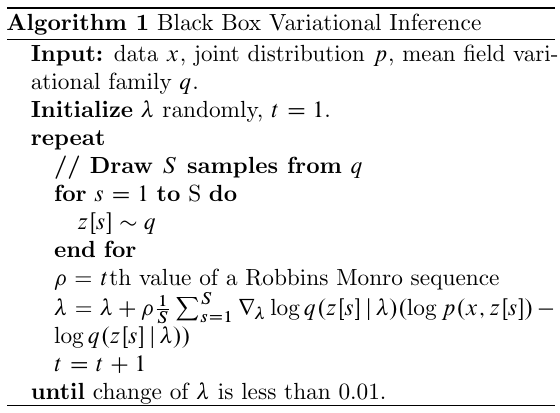
\includegraphics[width=0.85\textwidth]{VIBBVIAlgo1.png}
            \end{figure}
            \begin{itemize}
                \item Algorithm extends upon version 1 by using Rao-Blackwellization
                      and control-variates
            \end{itemize}
        \end{column}
        \begin{column}{0.48\textwidth}
            \begin{figure}
                \centering
                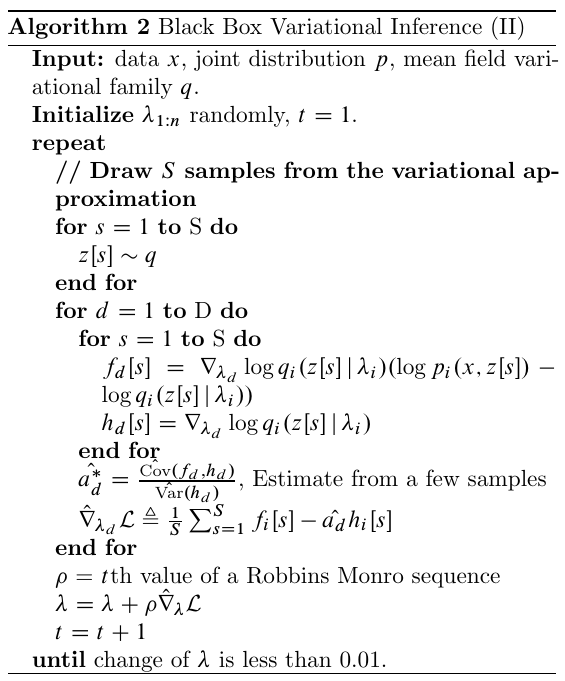
\includegraphics[width=0.85\textwidth]{VIBBVIAlgo2.png}
            \end{figure}
        \end{column}
    \end{columns}
\end{frame}


% Black-Box Variational Inference Slide 4
\begin{frame}[c]{Variational Approaches to Inference}{Black Box Variational Inference}
    \centering
    \begin{columns}[T]
        \begin{column}{0.48\textwidth}
            \begin{figure}
                \centering
                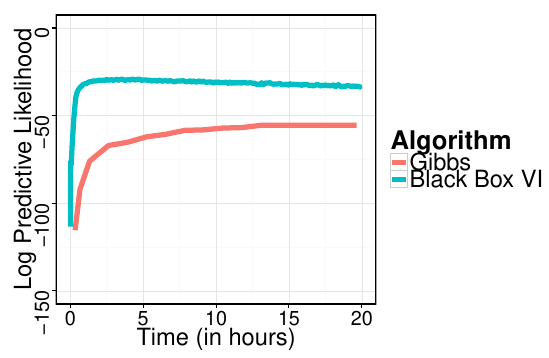
\includegraphics[width=0.85\textwidth]{ViBBVIPerformance1.png}
                \caption{Comparison between Metropolis-Hastings within Gibbs and Black Box Variational Inference}
            \end{figure}
        \end{column}
        \begin{column}{0.48\textwidth}
            \begin{figure}
                \centering
                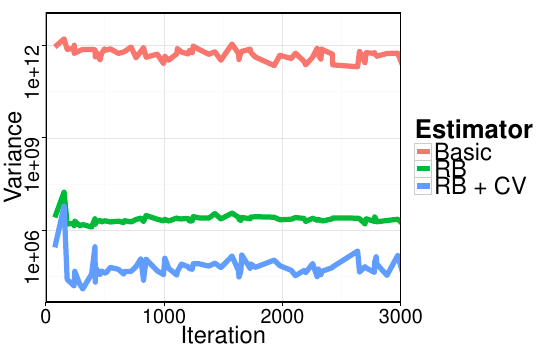
\includegraphics[width=0.8\textwidth]{VIBBVIPerformance2.png}
                \caption{Variance comparison between the different algorithms}
            \end{figure}
        \end{column}
    \end{columns}
\end{frame}



\subsubsection*{Automatic Differentiation Variational Inference}
% Automatic Differentiation Variational Inference Slide 1
\begin{frame}[c]{Variational Approaches to Inference}{Automatic Differentiation Variational Inference \footnote{Kucukelbir, A., Tran, D., Ranganath, R., Gelman, A. and Blei, D.M., 2017.
                                                                                                                Automatic differentiation variational inference. The Journal of Machine
                                                                                                                Learning Research, 18(1), pp.430-474.}
                                                                                                      \footnote{Kucukelbir, A., Ranganath, R., Gelman, A. and Blei, D., 2015. Automatic
                                                                                                                variational inference in Stan. In Advances in neural information processing
                                                                                                                systems (pp. 568-576).}}
    \centering
    \begin{itemize}
        \item Premise: Define your probabilistic model and your data, ADVI then performs inference in an
              automatic fashion
        \begin{itemize}
            \item ADVI generates the variational algorithm for the defined model
        \end{itemize}
        \item Steps of ADVI
        \begin{enumerate}
            \item Transform the latent space s.t. all latent variables are defined on the same space
            \item Recast gradient of variational objective as expectation over $q$
            \item Reparameterize the gradient in terms of a Gaussian
            \item Use noisy gradients to optimize the variational distribution
        \end{enumerate}
        \item Key ingredients herein are automatic differentiation capabilities in the probabilistic programming
              system and a library of transformations for step 1.
    \end{itemize}
\end{frame}


% Automatic Differentiation Variational Inference Slide 2
\begin{frame}[c]{Variational Approaches to Inference}{Automatic Differentiation Variational Inference}
    \centering
    \begin{itemize}
        \item Apply transformation s.t. the latent variables $\theta$ live in the real coordinate space $\mathbb{R}^{k}$
        \begin{equation*}
            p(x, \zeta) = p(x, T^{-1}(\zeta)) | \det J_{T^{-1}}(\zeta)|
        \end{equation*}
        \item The variational objective (ELBO) in the real coordinate space is then given by
        \begin{equation*}
            \mathcal{L}(\phi) = \mathbb{E}_{q(\zeta; \phi)} \left[ \log p(x, T^{-1}(\zeta)) + \log | \det J_{T^{-1}}(\zeta) | \right] + \mathbb{H}[q(\zeta; \phi)]
        \end{equation*}
        \item Applying elliptical standardization to make the expectation tractable
        \begin{equation*}
            \phi^{\star} = \underset{\phi}{\arg \max} \mathbb{E}_{N(\eta; 0, I)} \left[ \log p \left( x, T^{-1}(S^{-1}_{\phi}(\eta)) \right) + \log | \det J_{T^{-1}} \left( S^{-1}_{\phi}(\eta) \right) | \right] + \mathbb{H}[q(\zeta; \phi)]
        \end{equation*}
        \item Which can then be stochastically optimized
    \end{itemize}
\end{frame}


% Automatic Differentiation Variational Inference Slide 3
\begin{frame}[c]{Variational Approaches to Inference}{Automatic Differentiation Variational Inference}
    \centering
    \begin{figure}
        \centering
        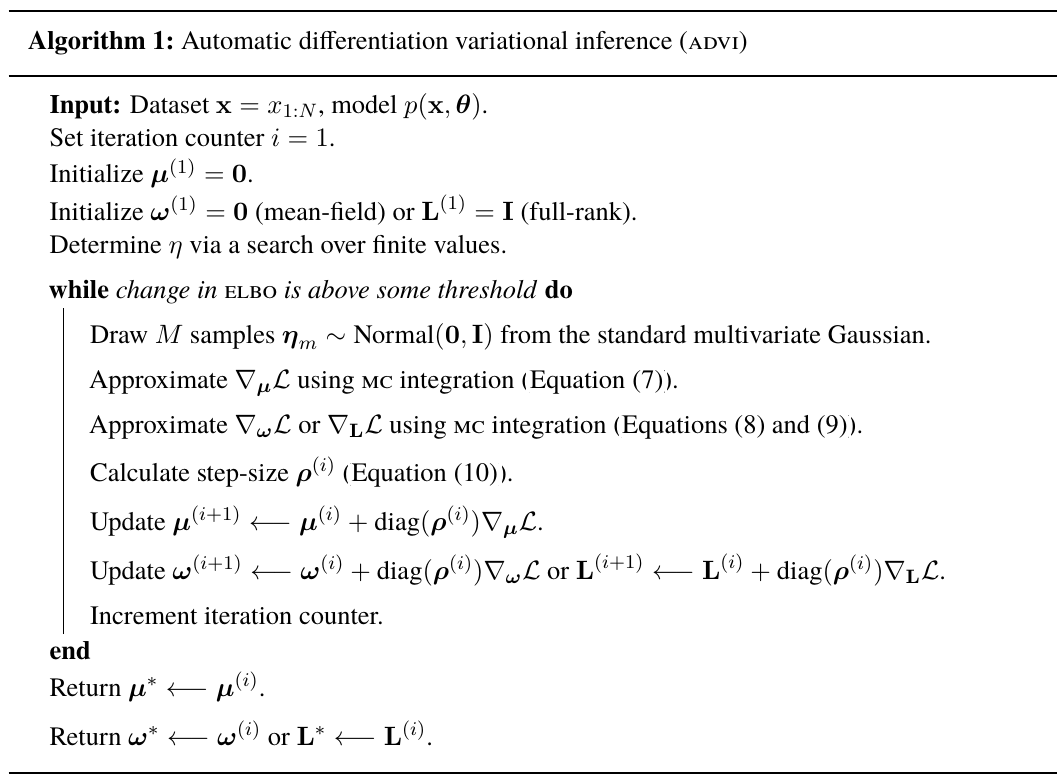
\includegraphics[width=0.65\textwidth]{VIADVIAlgo.png}
    \end{figure}
\end{frame}


% Automatic Differentiation Variational Inference Slide 4
\begin{frame}[c]{Variational Approaches to Inference}{Automatic Differentiation Variational Inference}
    \centering
    \begin{columns}[T]
        \begin{column}{0.4\textwidth}
            \begin{figure}
                \centering
                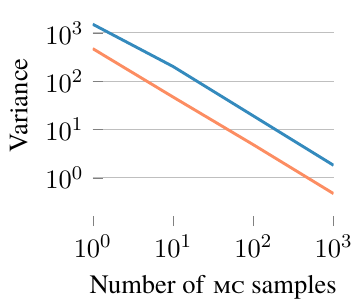
\includegraphics[width=0.95\textwidth]{VIADVIUnivariate.png}
                \caption{Univariate}
            \end{figure}
        \end{column}
        \begin{column}{0.58\textwidth}
            \begin{figure}
                \centering
                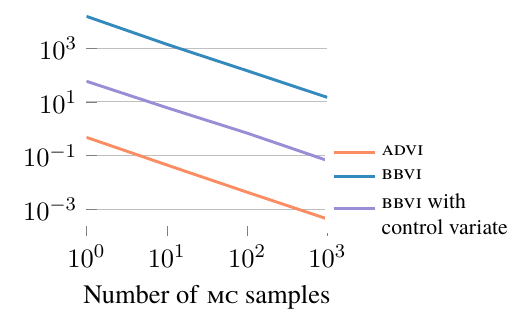
\includegraphics[width=0.9\textwidth]{VIADVIMultivariate.png}
                \caption{Multivariate}
            \end{figure}
        \end{column}
    \end{columns}
    \vspace{1cm}
    Comparison of gradient estimator variances
\end{frame}


% Automatic Differentiation Variational Inference Slide 5
\begin{frame}[c]{Variational Approaches to Inference}{Automatic Differentiation Variational Inference}
    \centering
    \begin{columns}[T]
        \begin{column}{0.4\textwidth}
            \begin{figure}
                \centering
                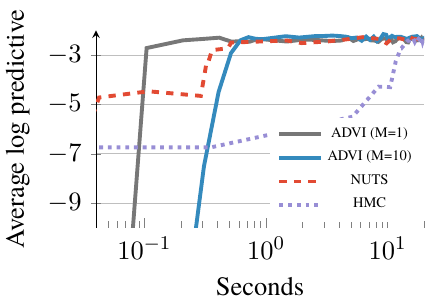
\includegraphics[width=\textwidth]{VIADVILinearRegression.png}
                \caption{Linear regression}
            \end{figure}
        \end{column}
        \begin{column}{0.58\textwidth}
            \begin{figure}
                \centering
                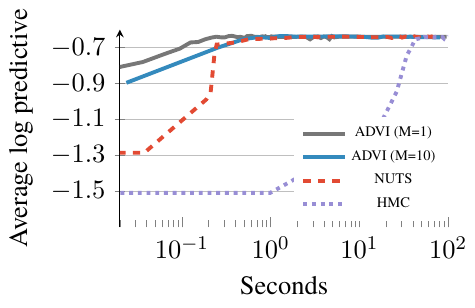
\includegraphics[width=0.75\textwidth]{ViADVIHierarchicalRegression.png}
                \caption{Hierarchical logistic regression}
            \end{figure}
        \end{column}
    \end{columns}
    \vspace{1cm}
    Held-out predictive accuracy results.
\end{frame}




% Probabilistic Programming Frameworks
\section{Probabilistic Programming Frameworks}


\subsection{Stan}
% Stan Slide 1: general introduction
\begin{frame}[c]{Stan \footnote{Carpenter, B., Gelman, A., Hoffman, M.D., Lee, D.,
                                Goodrich, B., Betancourt, M., Brubaker, M., Guo, J., Li, P.
                                and Riddell, A., 2017. Stan: A probabilistic programming
                                language. Journal of statistical software, 76(1).}}{Overview}
    \centering
    \begin{itemize}
        \item Stan is primarily aimed at statisticians and provides a full-fledged suite for them
              to express their statistical models and perform statistical inference
        \item Methods of inference provided:
        \begin{itemize}
            \item Hamiltonian Monte-Carlo
            \item no-U-turn sampler
            \item Automatic Differentiation Variational Inference
        \end{itemize}
        \item Defines its own separate DSL with interfaces for python, R, Matlab, Julia, State, Mathematica and the command-line
        \item Automatically differentiates the generative model using reverse-mode automatic differentiation
        \item Stan's core library in C++ with its interfaces to other languages makes it difficult to link to
              external simulators, the defined generatve model does furthermore get compiled, hence introducing
              a further layer of abstraction
    \end{itemize}
\end{frame}


% Stan Slide 2: Example Code
\begin{frame}[c]{Stan}{Syntax \footnote{Gelman, A., Lee, D. and Guo, J., 2015. Stan: A probabilistic programming language
                                        for Bayesian inference and optimization. Journal of Educational and Behavioral
                                        Statistics, 40(5), pp.530-543.}}
    \centering
    \begin{columns}[T]
        % Explanation of the code structure on the right
        \begin{column}{0.48\textwidth}
            \centering
            \vspace{1.5cm}
            \begin{itemize}
                \item Data block declares the data, which the program expects to receive
                \item Parameters block declared the unknown quantities, which are to be estimated
                \item Transformed parameters are functions of data and parameters
                \item Model block defines the computation of the log-posterior density
            \end{itemize}
        \end{column}
        % An example Stan model
        \begin{column}{0.48\textwidth}
            \centering
            \begin{figure}
                \centering
                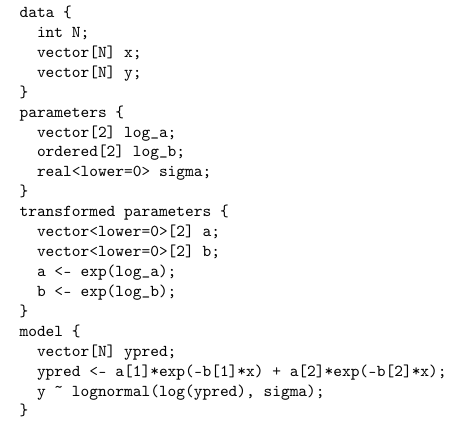
\includegraphics[width=0.9\textwidth]{StanExample.png}
            \end{figure}
        \end{column}
    \end{columns}
\end{frame}


% Stan Slide 3: Application Performance
\begin{frame}[c]{Stan}{Application Performance}
    \centering
    \begin{figure}
        \centering
        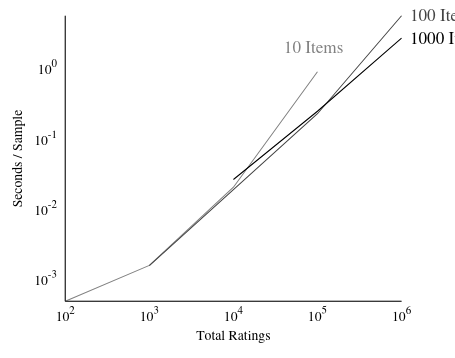
\includegraphics[width=0.4\textwidth]{STANSamplerperSecond.png}
    \end{figure}
    \begin{figure}
        \centering
        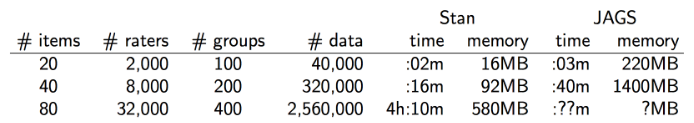
\includegraphics[width=0.75\textwidth]{STANImprovement.png}
    \end{figure}
\end{frame}


\subsection{Venture}
% Venture (2014) Slide 1: General Introduction
\begin{frame}[c]{Venture \footnote{Mansinghka, V., Selsam, D. and Perov, Y., 2014.
                                   Venture: a higher-order probabilistic programming platform
                                   with programmable inference. arXiv preprint arXiv:1404.0099.}
                         \footnote{Goodman, N., Mansinghka, V., Roy, D.M., Bonawitz, K. and Tenenbaum, J.B., 2012.
                                   Church: a language for generative models. arXiv preprint arXiv:1206.3255.}}{Overview}
    \centering
    \begin{itemize}
        \item Virtual machine for general-purpose probabilistic programming building on the ideas of Church,
              but enabling the user to specify custom inference strategies.
        \item Enables custom stochastic control flows through its stochastic procedure inferface
        \item Methods of inference provided include exact- and approximate inference:
        \begin{itemize}
            \item Metropolis-Hastings
            \item Hamiltonian Monte-Carlo
            \item Gibbs sampling
            \item Sequential Monte-Carlo
            \item Variational inference
            \item Inference programming is possible
        \end{itemize}
        \item Evolved into a modern version, called \textit{VentureScript}
        \item Able to link to external models, but not as easily as successor developments such as \textit{Gen}
    \end{itemize}
\end{frame}


% Venture Slide 2: Example Code
\begin{frame}[c]{Venture}{Syntax: Bayesian GP Optimization}
    \centering
    \begin{columns}[T]
        % description
        \begin{column}{0.38\textwidth}
            \centering
            \begin{itemize}
                \item Repeatedly samples from the response surface created by the Gaussian process (GP) surrogate to
                      reduce the number of function executions and discern the next point for function execution
                \item Then samples the function at said point to enrich our GP response surface
                \item Applies Metropolis-Hastings inference to the hyperparameters of the covariance function after
                      each function execution
            \end{itemize}
        \end{column}
        % Example code
        \begin{column}{0.6\textwidth}
            \centering
            \begin{figure}
                \centering
                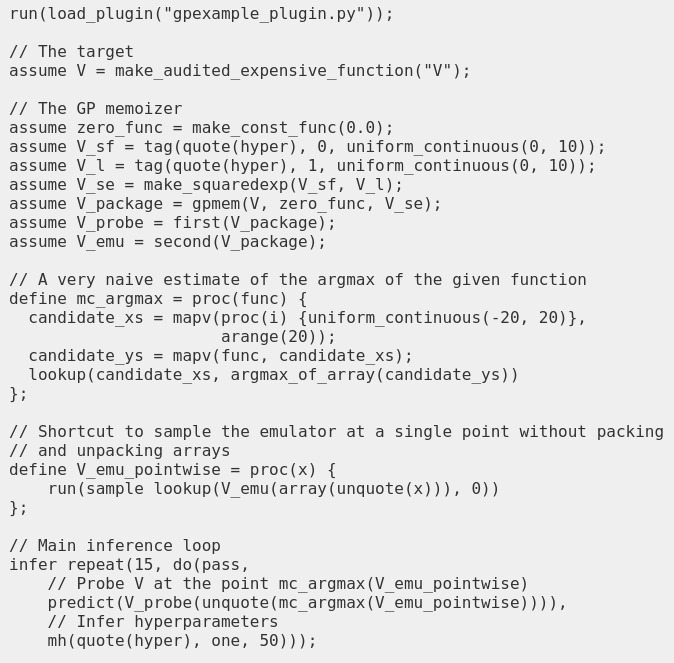
\includegraphics[width=0.8\textwidth]{VentureBayesOptExample.png}
            \end{figure}
        \end{column}
    \end{columns}
\end{frame}


% Venture Slide 3: Application Performance
\begin{frame}[c]{Venture}{Application Performance}
    \centering
    \begin{figure}
        \centering
        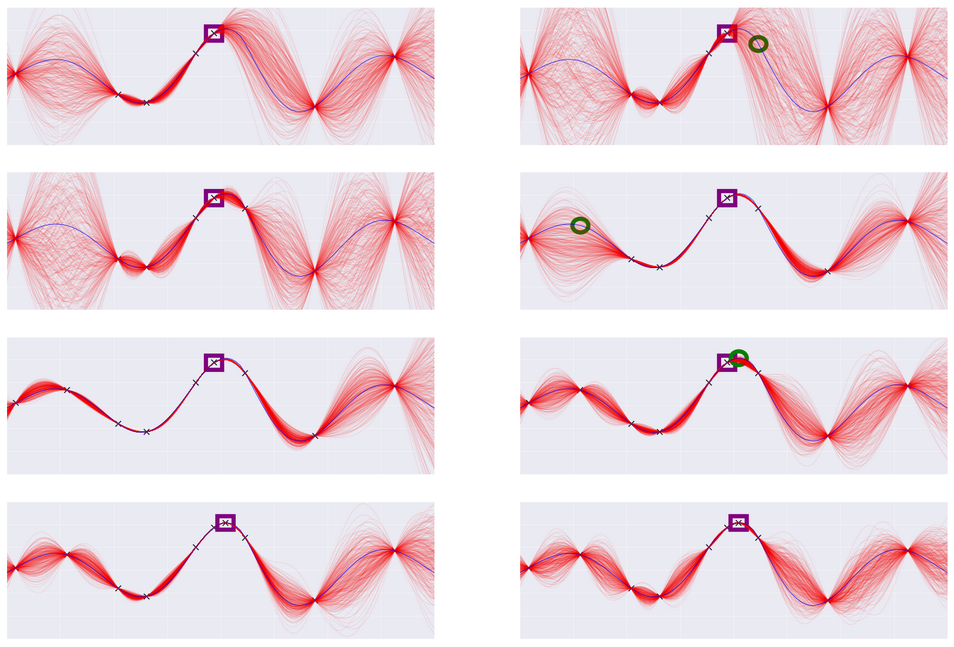
\includegraphics[width=0.7\textwidth]{VentureBayesOptExampleViz.png}
    \end{figure}
\end{frame}



\subsection{PyMC3}
% PyMC3 (2015) Slide 1: General Introdction
\begin{frame}[c]{PyMC3 \footnote{Salvatier, J., Wiecki, T.V. and Fonnesbeck, C., 2016. Probabilistic programming
                                 in Python using PyMC3. PeerJ Computer Science, 2, p.e55.}}{Overview}
    \centering
    \begin{itemize}
        \item Very well-suited for the construction of graphical models, but is not Turing-complete as it is unable to model
              recursive distributions, and programs that can write programs
        \item Provided inference routines:
        \begin{itemize}
            \item Hamiltonian Monte-Carlo
            \item No-U-Turn Sampler
            \item Sequential Monte-Carlo
            \item Automatic Differentiation Variational Inference
            \item Operator Variational Inference...
        \end{itemize}
        \item Provides first-class support for the incorporation of Gaussian processes for the construction of Bayesian nonparametric models
    \end{itemize}
\end{frame}


% PyMC3 Slide 2: Example Code
\begin{frame}[c]{PyMC3}{Syntax}
    \centering
    % Two columns, explanation on the left, example code on the right
    \begin{columns}[T]
        % Explanations
        \begin{column}{0.4\textwidth}
            \centering
            \begin{itemize}
                \item Constructing a toy neural network with 2 hidden layers of 5 neurons each
                \item Manual construction here, but PyMC3 is able to use Keras's API to Theano
                \item Mini-batches then accelerate convergence and allow the model to scale
            \end{itemize}
        \end{column}
        % Example code
        \begin{column}{0.58\textwidth}
            \centering
            \begin{figure}
                \centering
                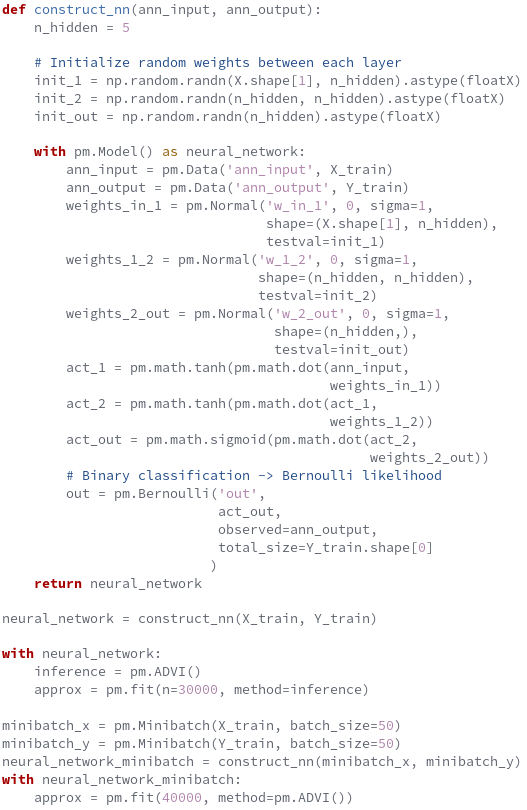
\includegraphics[width=0.54\textwidth]{PyMC3Syntax.png}
            \end{figure}
        \end{column}
    \end{columns}
\end{frame}


% PyMC3 Slide 3: Application Performance
\begin{frame}[c]{PyMC3}{Application Performance \footnote{Source: PyM3 Notebook on Variational Inference with Bayesian Neural Networks}}
    \centering
    % Two example performance pictures
    \begin{columns}[T]
        % Elbo improvements
        \begin{column}{0.48\textwidth}
            \centering
            \begin{figure}
                \centering
                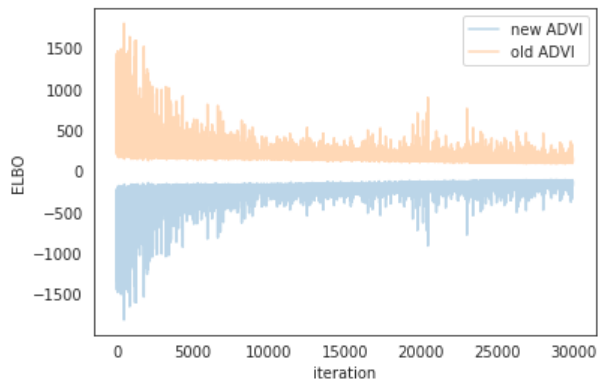
\includegraphics[width=\textwidth]{PyMC3ELBOAdvi.png}
                \caption{ADVI, 2073.86it/s}
            \end{figure}
        \end{column}
        % Mini-batch ELBO
        \begin{column}{0.48\textwidth}
            \centering
            \begin{figure}
                \centering
                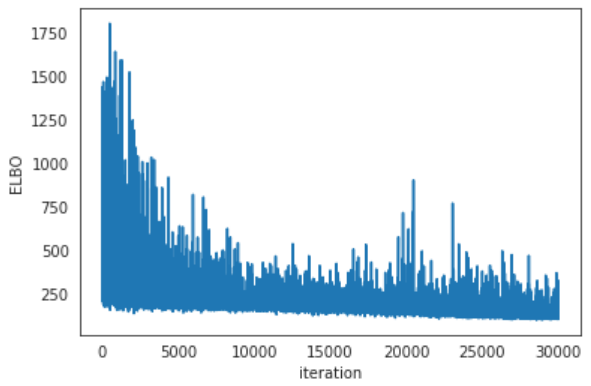
\includegraphics[width=\textwidth]{PyMC3ELBOMiniBatchAdvi.png}
                \caption{ADVI with mini-batch, 3586.77it/s}
            \end{figure}
        \end{column}
    \end{columns}
\end{frame}


\subsection{TensorFlow Probability}
% TensorFlow Probability (2017) Slide 1: General Introduction
\begin{frame}[c]{TensorFlow Probability \footnote{Dillon, J.V., Langmore, I., Tran, D., Brevdo, E., Vasudevan, S.,
                                                  Moore, D., Patton, B., Alemi, A., Hoffman, M. and Saurous, R.A., 2017.
                                                  Tensorflow distributions. arXiv preprint arXiv:1711.10604.}
                                        \footnote{Lao, J., Suter, C., Langmore, I., Chimisov, C., Saxena, A., Sountsov, P.,
                                                  Moore, D., Saurous, R.A., Hoffman, M.D. and Dillon, J.V., 2020. tfp. mcmc:
                                                  Modern Markov Chain Monte Carlo Tools Built for Modern Hardware. arXiv
                                                  preprint arXiv:2002.01184.}}{Overview}
    \centering
    \begin{itemize}
        \item Probabilistic reasoning and statistical analysis library built on top of TensorFlow with a full
              integration with deep models defined in TensorFlow, automatic differentiation support and scalability
              on accelerators
        \item Provided inference routines:
        \begin{itemize}
            \item Hamiltonian Monte-Carlo
            \item Langevin Monte-Carlo
            \item no-U-turn sampler
            \item Variational inference
        \end{itemize}
        \item Provides probably the most performant Markov Chain Monte-Carlo implementations to data, including
              multi-chain parallelism
    \end{itemize}
\end{frame}


% Tensorflow Probability Slide 2: Example Code
\begin{frame}[c]{TensorFlow Probability}{Syntax}
    \centering
    \begin{columns}[T]
        % Syntax 1
        \begin{column}{0.48\textwidth}
            \centering
            \begin{figure}
                \centering
                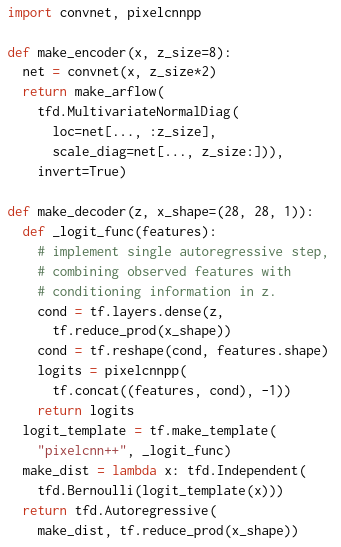
\includegraphics[width=0.6\textwidth]{TFProbSyntax1.png}
            \end{figure}
        \end{column}
        % Syntax 2
        \begin{column}{0.48\textwidth}
            \centering
            \begin{figure}
                \centering
                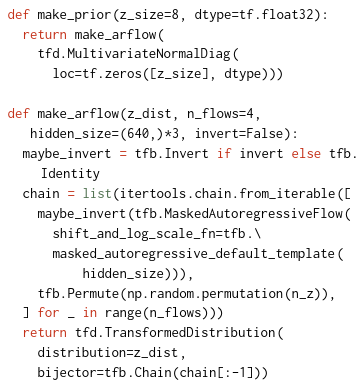
\includegraphics[width=0.7\textwidth]{TFProbSyntax2.png}
                \caption{SOTA with a PixelCNN++ decoder and autoregressive flows for encoder and prior.}
            \end{figure}
        \end{column}
    \end{columns}
\end{frame}


% Tensorflow Probability Slide 3: Application Performance
\begin{frame}[c]{TensorFlow Probability}{Application Performance}
    \centering
    \begin{figure}
        \centering
        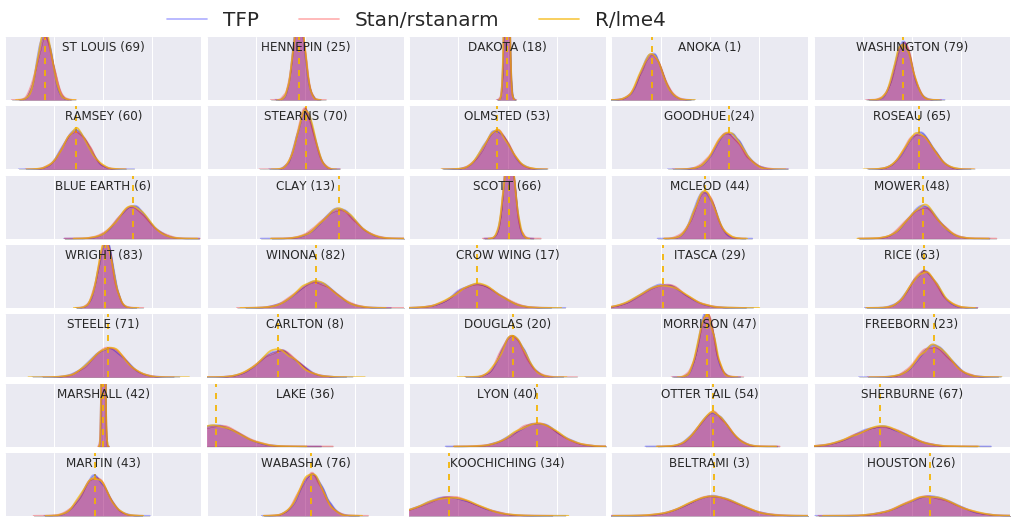
\includegraphics[width=0.8\textwidth]{TFProbAppPerformanceComparison.png}
        \caption{Linear Mixed-Effect Regression in TensorFlow Probability, R, and Stan \footnote{Source: TensorFlow Probability Tutorial}}
    \end{figure}
\end{frame}


\subsection{Pyro \& NumPyro}
% Pyro (2018) Slide 1: General introduction
\begin{frame}[c]{Pyro \footnote{Bingham, E., Chen, J.P., Jankowiak, M., Obermeyer, F., Pradhan, N., Karaletsos, T.,
                                Singh, R., Szerlip, P., Horsfall, P. and Goodman, N.D., 2019. Pyro: Deep universal
                                probabilistic programming. The Journal of Machine Learning Research, 20(1), pp.973-978.}
                \& NumPyro \footnote{Phan, D., Pradhan, N. and Jankowiak, M., 2019. Composable effects for flexible and
                                     accelerated probabilistic programming in NumPyro. arXiv preprint arXiv:1912.11554.}}{Overview}
    \centering
    \begin{itemize}
        \item Pyro \& NumPyro are both geared towards the definition of probabilistic programins in conjunction with state-of-the-art
              deep learning for large-data and high-dimensional models
        \item Methods of inference:
        \begin{itemize}
            \item Stochastic Variational Inference
            \item Importance Sampling
            \item Sequential Monte-Carlo
            \item Hamiltonian Monte-Carlo...
        \end{itemize}
        \item Saw a further iteration in NumPyro, which uses JAX \footnote{Bradbury, J., Frostig, R., Hawkins, P., Johnson, M.J., Leary, C., Maclaurin, D. and Wanderman-Milne, S., 2020. JAX: composable transformations of Python+ NumPy programs, 2018. URL http://github. com/google/jax, p.18.} as its backend to address accelerators
        \item Can link to simulator codes, but requires e.g. PPX bindings
    \end{itemize}
\end{frame}


% Pyro & NumPyro Slide 2: Example Code
\begin{frame}[c]{Pyro}{Syntax}
    \centering
    \begin{figure}
        \centering
        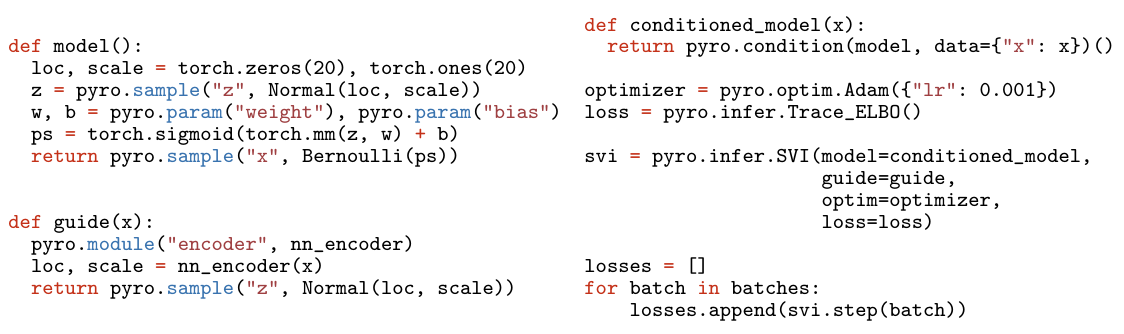
\includegraphics[width=\textwidth]{PyroSyntax.png}
        \caption{Pyro example with generative model, approximate posterior, constraint specification, and stochastic variational inference}
    \end{figure}
\end{frame}


% Pyro & NumPyro Slide 2: Example Code
\begin{frame}[c]{NumPyro}{Syntax}
    \centering
    \begin{columns}[T]
        % Syntax 1
        \begin{column}{0.48\textwidth}
            \centering
            \begin{figure}
                \centering
                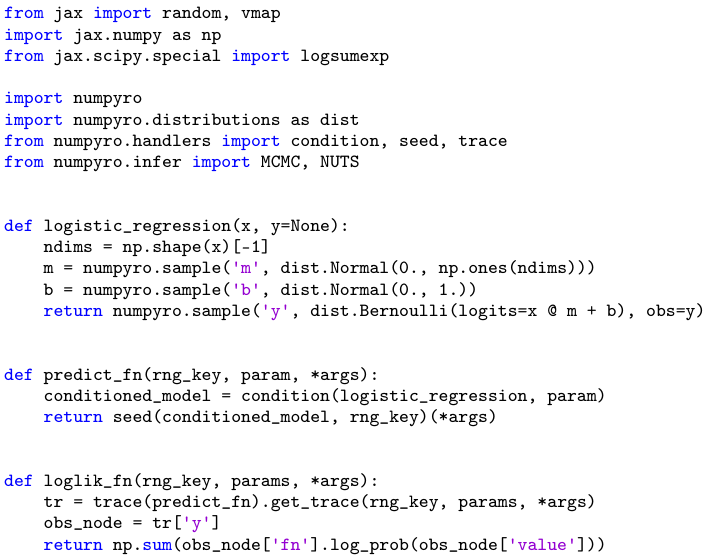
\includegraphics[width=\textwidth]{NumPyroSyntax1.png}
            \end{figure}
        \end{column}
        % Syntax 2
        \begin{column}{0.48\textwidth}
            \centering
            \begin{figure}
                \centering
                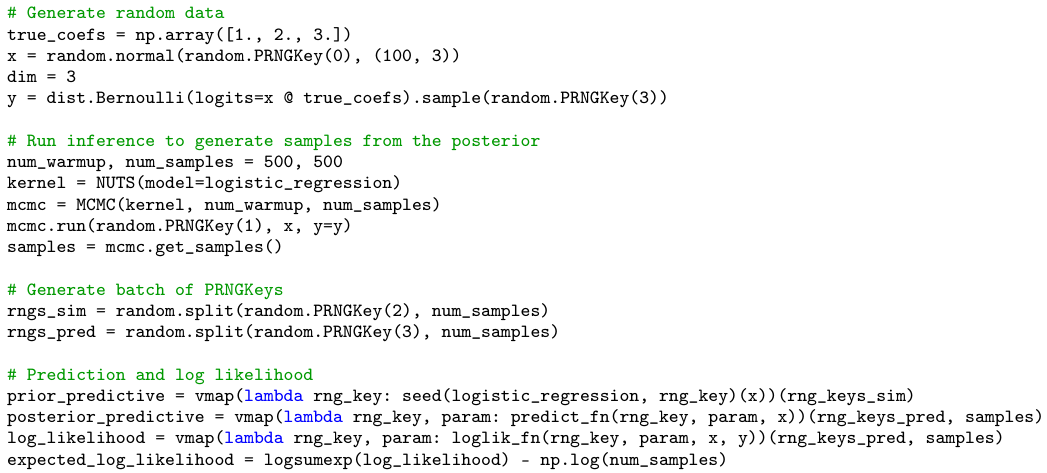
\includegraphics[width=\textwidth]{NumPyroSyntax2.png}
                \vspace{1cm}
                \caption{Example code syntax for vectorized sampling in a logistic regression example}
            \end{figure}
        \end{column}
    \end{columns}
\end{frame}


% Pyro & NumPyro Slide 3: Application Performance  -> Might want to add a second slide here for the performance of NumPyro
\begin{frame}[c]{Pyro \& NumPyro}{Application Performance}
    \centering
    \begin{columns}[T]
        % Comparison to Pyro and Stan
        \begin{column}{0.48\textwidth}
            \centering
            \vspace{0.5cm}
            \begin{figure}
                \centering
                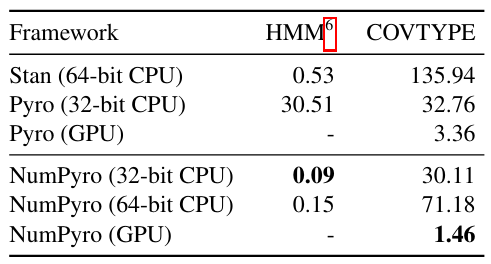
\includegraphics[width=0.8\textwidth]{NumPyroBenchmarking1.png}
                \caption{Time (ms) per leapfrog step in different frameworks}
            \end{figure}
        \end{column}
        % Time per effective sample scaling
        \begin{column}{0.48\textwidth}
            \centering
            \begin{figure}
                \centering
                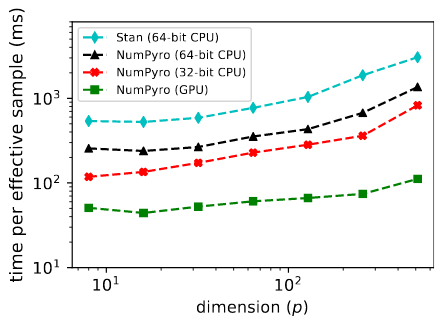
\includegraphics[width=0.8\textwidth]{NumPyroBenchmarking2.png}
                \caption{Time (ms) per effective sample for a sparse kernel interaction model as the
                     dimensionality of the dataset (p) is varied.}
            \end{figure}
        \end{column}
    \end{columns}
\end{frame}


\subsection{Edward2}
% Edward2 (2018/2019) Slide 1: General introduction
\begin{frame}[c]{Edward2 \footnote{Tran, D., Hoffman, M.W., Moore, D., Suter, C., Vasudevan, S. and Radul, A., 2018. Simple, distributed,
                                   and accelerated probabilistic programming. In Advances in Neural Information Processing Systems (pp. 7598-7609).}
                         \footnote{Tran, D., Dusenberry, M., van der Wilk, M. and Hafner, D., 2019. Bayesian layers: A module for neural network
                                   uncertainty. In Advances in Neural Information Processing Systems (pp. 14660-14672).}}{Overview}
    \centering
    \begin{itemize}
        \item A low-level approach to the embedding of probabilistic programming in the deep learning ecosystem, which
              hence runs directly on accelerator hardware and paves the way for larger scale models.
        \item Especially well-suited for the representation of uncertainty in neural network
        \item Provided inference routines:
        \begin{itemize}
            \item The same as TensorFlow probability
        \end{itemize}
        \item Highly efficient Monte-Carlo routines - use the same backend as TensorFlow probability
        \item Is able to utilize recent advances in XLA, such as sharding for large-scale models
        \item Removes many of the higher-level abstractions other languages benefit from
    \end{itemize}
\end{frame}


% Edward2 Slide 2: Example Code
\begin{frame}[c]{Edward2}{Syntax: Distributed Autoregressive Flow}
    \centering
    % Two columns for the example code and some minor explanation
    \begin{columns}[T]
        % Explanation
        \begin{column}{0.44\textwidth}
            \centering
            \begin{figure}
                \centering
                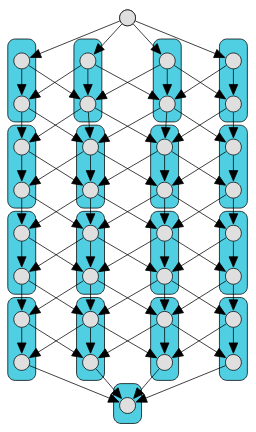
\includegraphics[width=0.55\textwidth]{Edward2Distributed.png}
            \end{figure}
        \end{column}
        % Syntax
        \begin{column}{0.56\textwidth}
            \centering
            \begin{figure}
                \centering
                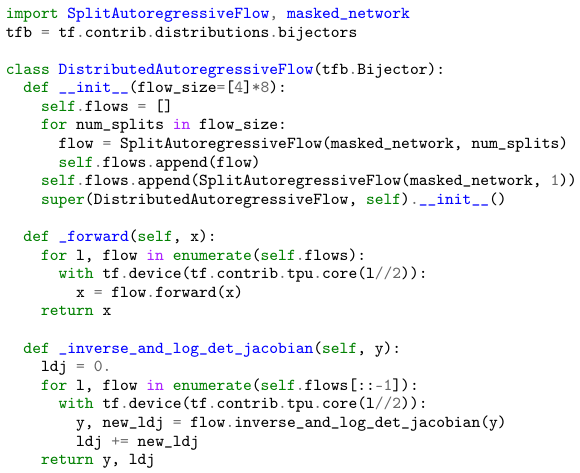
\includegraphics[width=0.85\textwidth]{Edward2Syntax.png}
            \end{figure}
        \end{column}
    \end{columns}
\end{frame}


% Edward2 Slide 3: Application Performance
\begin{frame}[c]{Edward2}{Application Performance}
    \centering
    % Two columns for 3 pictures overall
    \begin{columns}[T]
        % 2 picture columns
        \begin{column}{0.48\textwidth}
            \centering
            \begin{figure}
                \centering
                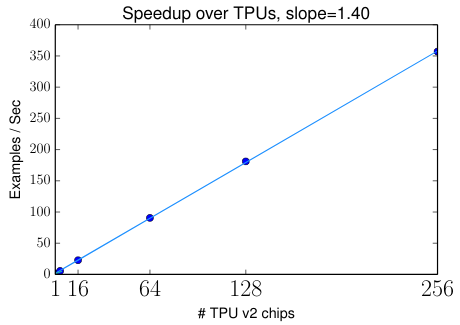
\includegraphics[width=0.65\textwidth]{Edward2Vector-QuantizedVAE.png}
            \end{figure}
            \begin{figure}
                \centering
                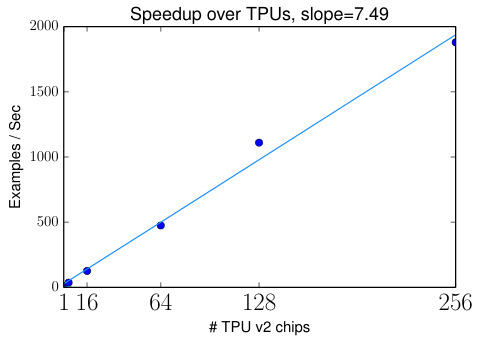
\includegraphics[width=0.65\textwidth]{Edward2ImageTransformer.png}
            \end{figure}
        \end{column}
        % Performance comparison column
        \begin{column}{0.48\textwidth}
            \centering
            \begin{figure}
                \centering
                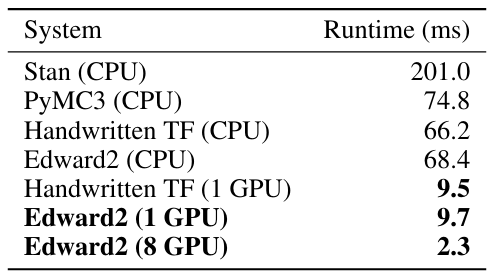
\includegraphics[width=0.7\textwidth]{Edward2PerformanceComparison.png}
            \end{figure}
            \vspace{0.5cm}
            \begin{itemize}
                \item[\textbf{(top-left):}] Vector-Quantized VAE on 64x64 ImageNet
                \item[\textbf{(bottom-left):}] Image Transformer on 256x256 CelebA-HQ
                \item[\textbf{(top-right):}] Time per leapfrog step for No-U-Turn Sample in Bayesian logistic regression 
            \end{itemize}
        \end{column}
    \end{columns}
\end{frame}


\subsection{Gen}
% Gen (2019) Slide 1: General introduction
\begin{frame}[c]{Gen \footnote{Cusumano-Towner, M.F., Saad, F.A., Lew, A.K. and Mansinghka, V.K., 2019, June. Gen: a general-purpose
                               probabilistic programming system with programmable inference. In Proceedings of the 40th ACM SIGPLAN
                               Conference on Programming Language Design and Implementation (pp. 221-236).}
                     \footnote{Cusumano-Towner, M., Lew, A.K. and Mansinghka, V.K., 2020. Automating Involutive MCMC using
                               Probabilistic and Differentiable Programming. arXiv preprint arXiv:2007.09871.}}{Overview}
    \centering
    \begin{itemize} % Mention the programmable inference to push the boundaries of prob prog here
        \item Introduces multiple further abstractions, which differ from the other probabilistic programming frameworks
              as it relies on the abstraction of generative functions and a directly expandable infernece library
        \begin{itemize}
            \item Especially geared towards computer vision and robotics
        \end{itemize}
        \item Provides a dynamic, as well as a static DSL
        \item Provided inference routines:
        \begin{itemize}
            \item Hamiltonian Monte-Carlo
            \item Importance Sampling
            \item Sequential Monte-Carlo
            \item Black-Box Variational Inference...
        \end{itemize}
        \item Able to link to simulators and amenable to metaprogramming
    \end{itemize}
\end{frame}


% Gen Slide 2: Difference to other probabilistic programming system
\begin{frame}[c]{Gen}{Programmable Inference}
    \centering
    \begin{figure}
        \centering
        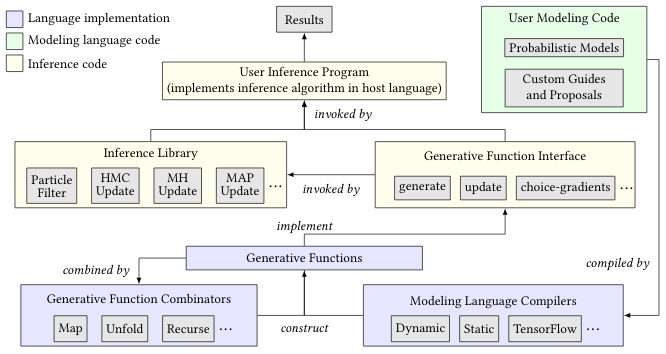
\includegraphics[width=0.7\textwidth]{GenSpecialArchitecture.png}
        \caption{Gen's layout, which introduces further abstractions to go beyond current
                 probabilistic programming systems.}           
    \end{figure}
\end{frame}

% Gen Slide 3: Example Code
\begin{frame}[c]{Gen}{Syntax: Body Pose Inference}
    \centering
    % Two columns of code
    \begin{columns}[T]
        % Model and neural net definition
        \begin{column}{0.48\textwidth}
            \centering
            \begin{figure}
                \centering
                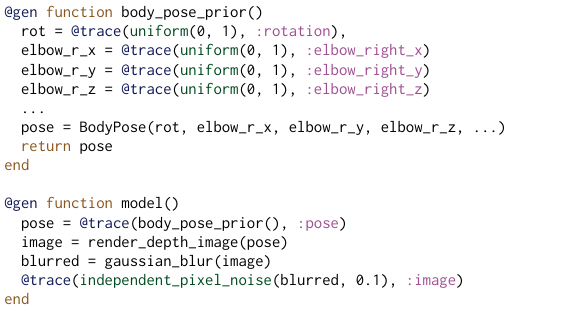
\includegraphics[width=\textwidth]{GenModelDML.png}
            \end{figure}
            \begin{figure}
                \centering
                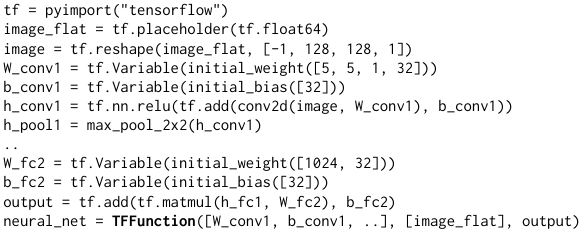
\includegraphics[width=\textwidth]{GenBodyPoseTML.png}
            \end{figure}
        \end{column}
        % Custom proposal and importance sample
        \begin{column}{0.48\textwidth}
            \centering
            \begin{figure}
                \centering
                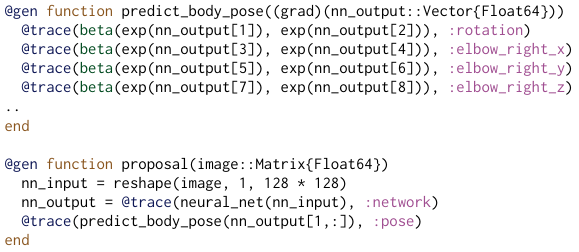
\includegraphics[width=\textwidth]{GenBodyPoseProposalDML.png}
            \end{figure}
            \begin{figure}
                \centering
                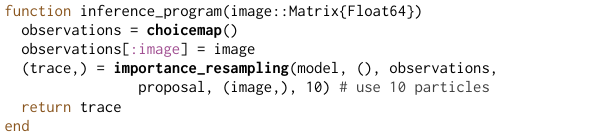
\includegraphics[width=\textwidth]{GenBodyPoseInference.png}
                \caption{Code and evaluation for body pose inference.}
            \end{figure}
        \end{column}
    \end{columns}
\end{frame}


% Gen Slide 4: Application perforance
\begin{frame}[c]{Gen}{Application Performance}
    \centering
    \begin{columns}[T]
        % Performance comparison 1
        \begin{column}{0.48\textwidth}
            \centering
            \begin{figure}
                \centering
                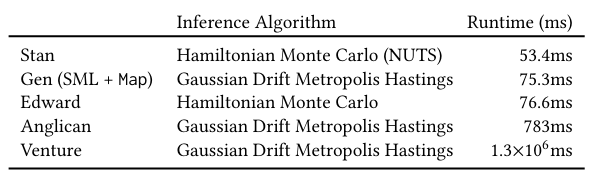
\includegraphics[width=\textwidth]{GenInferenceinCollapsedModel.png}
                \caption{Comparison of inference in collapsed model.}
            \end{figure}
            \begin{figure}
                \centering
                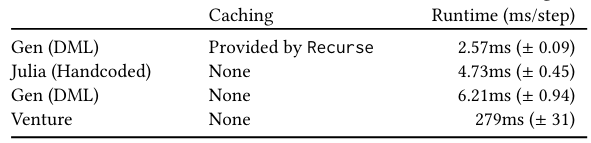
\includegraphics[width=\textwidth]{GenGPStructureLearning.png}
                \caption{Comparison on gaussian process structure learning.}
            \end{figure}
        \end{column}
        % Performance comparison 2
        \begin{column}{0.48\textwidth}
            \centering
            \begin{figure}
                \centering
                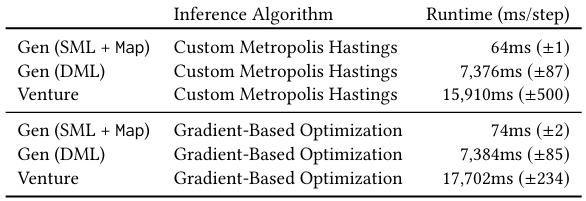
\includegraphics[width=\textwidth]{GenInferenceUncollapsedModel.png}
                \caption{Comparison of inference in uncollapsed model. Including the visibly
                         much fast static DSL of Gen in comparison with the dynamic DSL.}
            \end{figure}
        \end{column}
    \end{columns}
\end{frame}


\subsection{PyProb}
% PyProb (2019) Slide 1: General introduction
\begin{frame}[c]{PyProb \footnote{Baydin, A.G., Shao, L., Bhimji, W., Heinrich, L., Naderiparizi, S., Munk, A., Liu, J., Gram-Hansen, B.,
                                  Louppe, G., Meadows, L. and Torr, P., 2019. Efficient probabilistic inference in the quest for physics
                                  beyond the standard model. In Advances in neural information processing systems (pp. 5459-5472).}}{Overview}
    \centering
    \begin{itemize}
        \item Custom-made for concurrent workflows with HPC simulations through the PPX protocol based on flatbuffers, and tested on supercomputers
        \item Provided inference routines:
        \begin{itemize}
            \item Markov Chain Monte-Carlo
            \item Importance sampling
            \item Importance sampling with inference compilation
        \end{itemize}
        \item Made for distributed execution across large machines with distributed PyTorch providing the MPI-fuelled backend
        \item Intel-optimized PyTorch backend version
        \begin{itemize}
            \item Possibly not the greatest performance on the heterogeneous machines of the future $\longrightarrow$ Is XLA possibly the safer bet for
                  such a codebase?
        \end{itemize}
    \end{itemize}
\end{frame}


% PyProb Slide 2: Example Code
\begin{frame}[c]{PyProb}{Syntax}
    \centering
    \begin{columns}[T]
        % Syntax 1
        \begin{column}{0.48\textwidth}
            \centering
            \begin{figure}
                \centering
                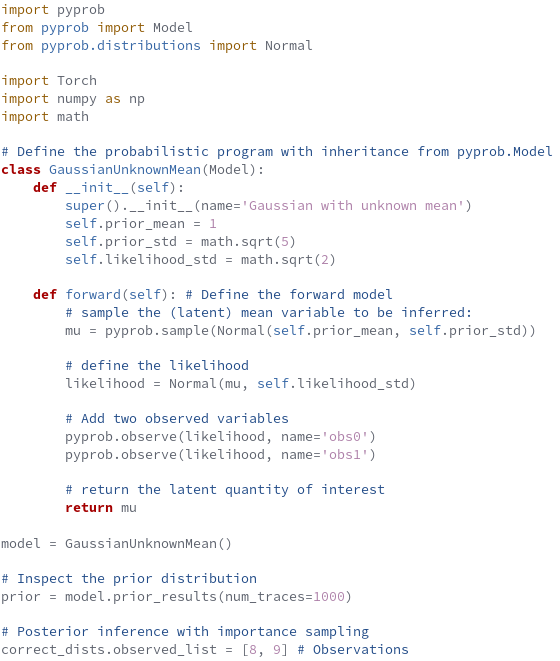
\includegraphics[width=0.8\textwidth]{PyProbSyntax1.png}
            \end{figure}
        \end{column}
        % Syntax 2
        \begin{column}{0.48\textwidth}
            \centering
            \begin{figure}
                \centering
                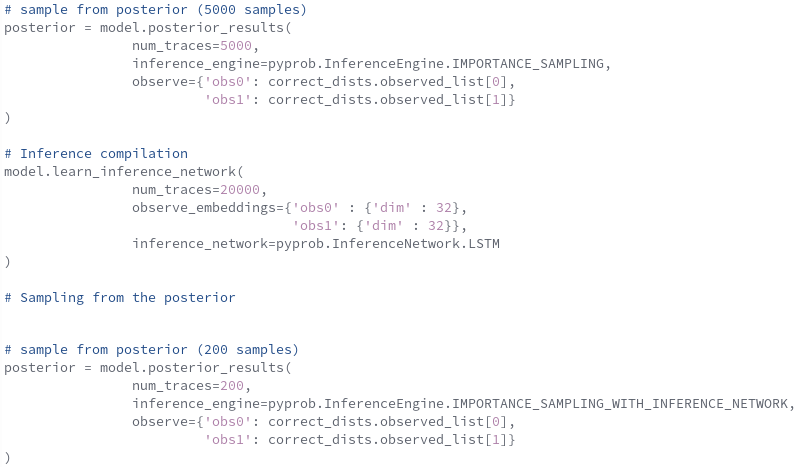
\includegraphics[width=\textwidth]{PyProbSyntax2.png}
                \caption{Probabilistic inference on a Gaussian with unknown mean}
            \end{figure}
        \end{column}
    \end{columns}
\end{frame}


% PyProb Slide 3: Application performance
\begin{frame}[c]{PyProb}{Application Performance}
    \centering
    \begin{columns}[T]
        % Weak scaling on Cori
        \begin{column}{0.48\textwidth}
            \centering
            \begin{figure}
                \centering
                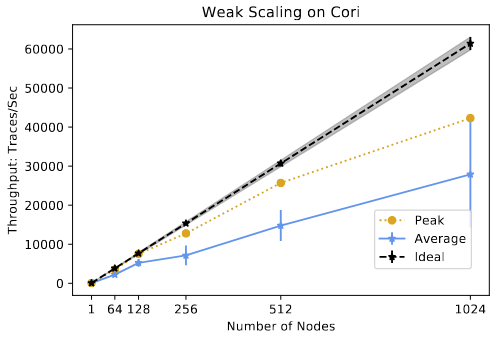
\includegraphics[width=\textwidth]{PyProbScalingCori.png}
            \end{figure}
        \end{column}
        % Weak scaling on Edison
        \begin{column}{0.48\textwidth}
            \centering
            \begin{figure}
                \centering
                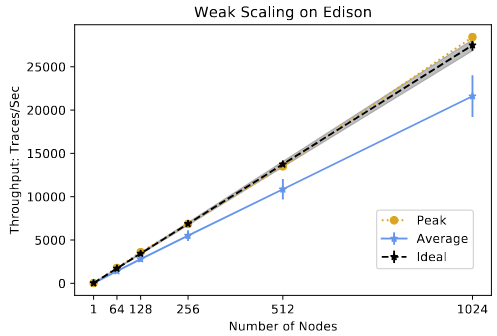
\includegraphics[width=\textwidth]{PyProbScalingEdison.png}
            \end{figure}
        \end{column}
    \end{columns}
\end{frame}


\subsection{Turing}
% Turing (2018) Side 1: General introduction
\begin{frame}[c]{Turing \footnote{Ge, H., Xu, K. and Ghahramani, Z., 2018, March. Turing: A Language for Flexible
                                  Probabilistic Inference. In International Conference on Artificial Intelligence
                                  and Statistics (pp. 1682-1690).}}{Overview}
    \centering
    \begin{itemize}
        \item Turing is a high-level probabilistic programming language, which provides extremely solid
              inference routines to the researcher
        \item Seamless compatibility with the entire Julia scientific machine learning stack enables many
              interesting cases
        \begin{itemize}
            \item More on this later!
        \end{itemize}
        \item Provided inference algorithms:
        \begin{itemize}
            \item Hamiltonian Monte-Carlo
            \item No-U-Turn Sampler
            \item Automatic Differentiation Variational Inference
            \item Normalizing Flows
        \end{itemize}
        \item Different inference subroutines can be composed, hence allowing for individual inference subroutines
    \end{itemize}
\end{frame}


% Turing Slide 2: Example code
\begin{frame}[c]{Turing}{Syntax}
    \centering
    % Explanation on the left, code on the right
    \begin{columns}[T]
        % Explanation
        \begin{column}{0.4\textwidth}
            \centering
            \begin{itemize}
                \item The \textit{model} macro identifies our function as a probabilistic model
                      to Turing, i.e. registers it for eventuel forward- and reverse-mode gradients
                \item $\theta, \phi$ \& $z$ denote model parameters
                \item K, M, N, d, $\beta$, \& $\alpha$ denote hyperparameters
                \item w denotes the observed data
            \end{itemize}
        \end{column}
        % Syntax example
        \begin{column}{0.58\textwidth}
            \centering
            \begin{figure}
                \centering
                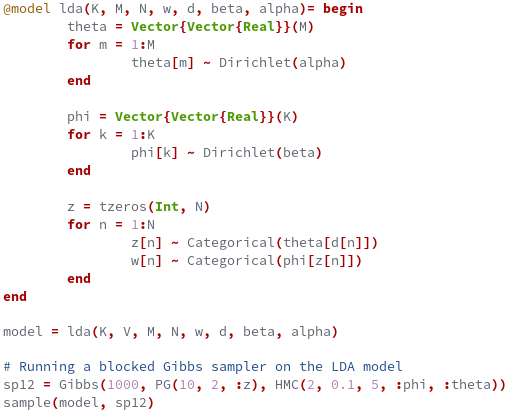
\includegraphics[width=\textwidth]{TuringSyntax.png}
            \end{figure}
        \end{column}
    \end{columns}
\end{frame}


% Turing Slide 3: Application performance
\begin{frame}[c]{Application performance}
    \centering
    % Densitiy estimation example
    \begin{figure}
        \centering
        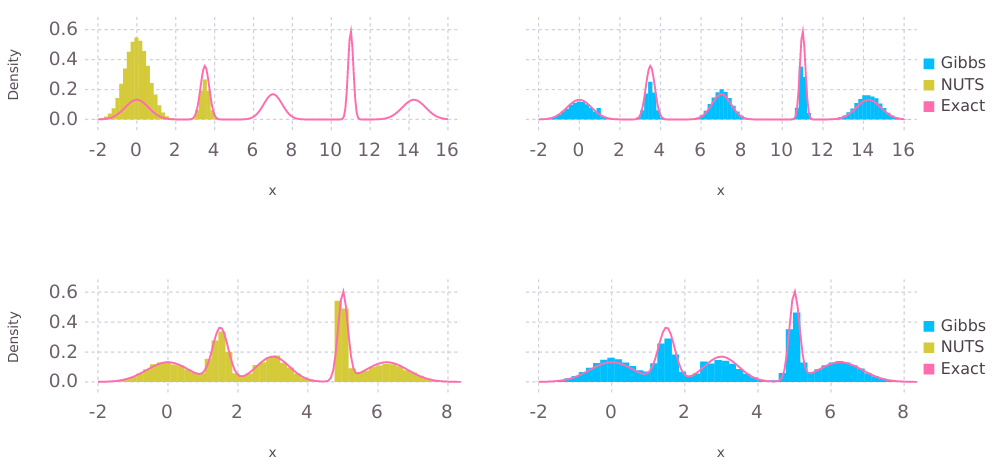
\includegraphics[width=0.5\textwidth]{TuringAppPerformanceNUTSvsGibbs.png}
        \caption{Performance on a Gaussian mixture model}
    \end{figure}
    % HMC Performance
    \begin{figure}
        \centering
        \includegraphics[width=0.7\textwidth]{TuringPerformancevsStanHMC.png}
        \caption{Runtime comparison for Turing vs Stan for HMC.}
    \end{figure}
\end{frame}


% Summary in matrix form
\begin{frame}[c]{Probabilistic Programming Frameworks}{Summary}
    \centering
    \begin{itemize}
        \item There are many vectors we ought to consider when deciding upon a probabilistic programming framework
        \begin{itemize}
            \item Can I represent my problem in the respectve DSL, or do I require a full-fledged language?
            \begin{itemize}
                \item Python- or Julia-based probabilistic programming system
            \end{itemize}
            \item Do I require support for meta-programming?
            \begin{itemize}
                \item Julia- or Lisp-based probabilistic programming system
            \end{itemize}
            \item How scalable and accelerator-portable is my framework supposed to be?
            \begin{itemize}
                \item Probabilistic programming system with an XLA-backend
            \end{itemize}
            \item Do I want to interface with simulators?
            \begin{itemize}
                \item Gen, or PyProb
            \end{itemize}
            \item Do I want to have inference programming capability?
            \begin{itemize}
                \item Gen, or Venture
            \end{itemize}
            \item How high- or low-level do I want to program?
        \end{itemize}
    \end{itemize}
\end{frame}



% Practical Introduction to Turing
\section{Practical Introduction to a Probabilistic Programming Framework}


% Slide leading over to the Jupyter notebook
\begin{frame}[c]{Introduction to Turing}
    \centering
    \begin{itemize}
        \item We will do our first steps in a probabilistic programming framework with Turing covering
        \begin{itemize}
            \item The modelling syntax
            \item Sampling
            \item Accessing the trace
            \item Automatic differentiation
            \item Working with dynamic Hamiltonian Monte-Carlo
        \end{itemize}
        \item All content can be accessed in the Jupyter notebook \textbf{IntrotoTuring.ipynb}
    \end{itemize}
\end{frame}


% Extension to a more complex example
\section{Extending the ideas to a more complex examples}


% Slide leading over to the Jupyter notebook
\begin{frame}[c]{More Complex Example in Turing}{Model-based inference for causal effects in completely randomized experiments}
    \centering
    \begin{itemize}
        \item Expanding on the simple syntax we will now move to a more complex case:
        \begin{itemize}
            \item Starting with a Bayesian perspective on causal inference
            \item Assignment mechanisms
            \item Posterior inference
        \end{itemize}
        \item All content can be accessed in the Jupyter notebook \textbf{MBInferenceforCausalEffects.ipynb}
    \end{itemize}
\end{frame}






%
%\AERbeamerSetFooterText{References}%
%\begin{frame}[allowframebreaks]{References}%
%    \printbibliography[heading=none]%
%\end{frame}%
%
% End with titlepage
%\AERbeamerTitlePageDefault%
%
%
\end{document}%
%
%
